\documentclass[uplatex,dvipdfmx]{jsarticle}
\usepackage{amssymb}
\usepackage{amsmath}
\usepackage{amsthm}
\usepackage{framed}
\usepackage{braket}
\usepackage{bm}
\usepackage{mathrsfs}
\usepackage{mathabx}
\usepackage{accents}
\usepackage{tocloft}
\usepackage{graphicx}
\usepackage{tikz}
\usepackage{url}
\usepackage{color}
\usepackage{xifthen}
\usepackage{xcolor}
\usepackage{framed}
\usepackage{mathtools}
\usepackage[explicit]{titlesec}
\usepackage[normalem]{ulem}
\usepackage{stmaryrd}
\usepackage{hyperref}
\usepackage{pxjahyper}
\usepackage[backend=biber,style=numeric,sorting=none,doi=false,isbn=false,url=false]{biblatex}
\addbibresource{bib.bib}


\usetikzlibrary{positioning}
\usetikzlibrary{calc}
\usetikzlibrary{decorations.pathreplacing}
\usetikzlibrary{cd}

\newcommand{\scrN}{\mathcal{N}}
\newcommand{\scrC}{\mathcal{C}}
\newcommand{\N}{\mathbb{N}}
\newcommand{\Z}{\mathbb{Z}}
\newcommand{\Q}{\mathbb{Q}}
\newcommand{\R}{\mathbb{R}}
\newcommand{\C}{\mathbb{C}}
\newcommand{\PP}{\mathcal{P}}
\newcommand{\range}{\operatorname{ran}}
\newcommand{\dom}{\operatorname{dom}}
\newcommand{\Func}{\operatorname{Func}}
\newcommand{\intr}{\operatorname{int}}
\newcommand{\cl}{\operatorname{cl}}
\newcommand{\RO}{\operatorname{RO}}
\newcommand{\append}{{}^\frown}
\newcommand{\Ordinals}{\mathrm{On}}
\newcommand\forces{\Vdash}
\newcommand\notforces{\nVdash}
\renewcommand\emptyset{\varnothing}
\renewcommand\subset{\subseteq}

\newcommand{\truth}[1] {\llbracket #1 \rrbracket}
\newcommand{\textwospace}[1] {\text{#1} \hspace{-0.01cm}}
\newcommand{\truthtext}[1] {\llbracket \text{#1} \hspace{-0.01cm} \rrbracket}

\newcommand{\needtocheck}[1][]{%
	\ifthenelse{\equal{#1}{}}{%
		\textcolor{blue}{[要チェック]}%
	}{%
		\textcolor{blue}{[要チェック: #1]}%
	}%
}


\definecolor{TodoRed}{HTML}{c41c10}

\newcommand{\todo}[1][]{%
	\ifthenelse{\equal{#1}{}}{%
		\textcolor{TodoRed}{[TODO]}%
	}{%
		\textcolor{TodoRed}{[TODO: #1]}%
	}%
}

\theoremstyle{definition}
\newtheorem{thm}{定理}
\newtheorem*{thm*}{定理}
\newtheorem{defi}[thm]{定義}
\newtheorem*{defi*}{定義}
\newtheorem{lem}[thm]{補題}
\newtheorem*{lem*}{補題}
\newtheorem{fact}[thm]{事実}
\newtheorem*{fact*}{事実}
\newtheorem*{formula*}{公式}
\newtheorem{prop}[thm]{命題}
\newtheorem*{prop*}{命題}
\newtheorem{exm}[thm]{例}
\newtheorem{rmk}[thm]{注意}
\newtheorem*{rmk*}{注意}
\newtheorem{cor}[thm]{系}
\newtheorem*{cor*}{系}
\newtheorem*{notation*}{記法}
\renewcommand{\proofname}{証明}
\newenvironment{claim}[1]{\par\noindent\underline{主張:}\space#1}{}
\newenvironment{claimproof}[1]{\par\noindent∵) \space#1}{\hfill //}

\title{集合論のブール代数値モデルおよびハイティング代数値モデル}
\date{2020年8月30日 作成 \\ 2023年3月23日 最終更新}
\author{でぃぐ}

\begin{document}
\maketitle

\begin{abstract}
1963年コーエンは連続体仮説の独立性を示すために強制法を編み出した.それはソロヴェイ,スコット,ヴォペンカによって即座にブール代数値モデルという方法に一般化された.そこで使われたブール代数をもっと広げてハイティング代数を使ったら直観主義集合論のモデルが出来る.この発表では実際にブール代数値モデルおよびハイティング代数値モデルによって集合論のモデルを作る.
\end{abstract} 

\tableofcontents

\section{イントロダクション}

普通,$x, y$という集合二つがあったら$x = y$という主張は真か偽のどちらかである.半分くらい真で半分くらい偽というのはない.
しかし,命題の真理値が真と偽の中間でありえるような世界を考えたらどうだろう.
つまり$\{0, 1\}$という2元ブール代数の代わりに一般の完備ブール代数を考えてそこの元を真理値にとるようにする世界を考えるのである.
たとえば,閉区間$[0, 1]$の正則開集合全体のなす完備ブール代数を考え,$x = y$の真理値,あるいは確率は区間$(0.2, 0.4)$である,という具合に.
確率という言葉は実数値をとるように聞こえるがそうではなく,ブール代数の元を確率と呼んでいる.
さて,こうして集合論のブール代数値モデルが作られる.
実はこれは,コーエンが連続体問題を解決するために編み出した強制法の定式化の一つなのである.

適切な完備ブール代数を選べば,ZFCで証明できるわけでもないのに,ある命題の真理値を$1$にすることができる.
たとえば,位相空間$2^{\omega_2}$の正則開集合のなすブール代数では$2^{\aleph_0} \ge \aleph_2$の真理値は$1$となっている.

また,完備ブール代数の代わりに完備ハイティング代数を考えれば,直観主義の集合論のモデルも作ることができる.

\section{予備知識}

\subsection{ZFC}

唯一の非論理記号$\in$を持つ一階の言語の上で次の公理群を考え,これをZFCという.

\begin{enumerate}
    \item 外延性公理 $\forall A, B\ (\forall x\ (x \in A \leftrightarrow x \in B) \to A = B)$
    \item 分離公理 論理式$\varphi$ごとに$\forall \vec{t}\ \forall A\ \exists B\ \forall x\ (x \in B \leftrightarrow x \in A \land \varphi(A, \vec{t}, x))$
    \item 対公理 $\forall a, b\ \exists C\ \forall x\ ((x = a \lor x = b) \leftrightarrow x \in C)$
    \item 和集合公理 $\forall \mathcal{A}\ \exists B\ \forall x\ (\exists Y\ (x \in Y \land Y \in \mathcal{A}) \leftrightarrow x \in B)$
    \item 冪集合公理 $\forall A\ \exists \mathcal{B}\ \forall X\ (X \subset A \leftrightarrow X \in \mathcal{B})$
    \item 無限公理 $\exists A\ (\emptyset \in A \land \forall x \in A\ (x \cup \{x\} \in A))$
    \item 正則性公理 論理式$\varphi$ごとに$\forall \vec{t}\ (\forall x\ (\forall y \in x\ \varphi(y, \vec{t}) \to \varphi(x, \vec{t})) \to \forall x\ \varphi(x, \vec{t}))$
    \item 置換公理 論理式$\varphi$ごとに$\forall \vec{t}\ \forall A\ (\forall x\in A\ \exists y\ \varphi(x, y, \vec{t}) \to \exists B\ \forall x \in A\ \exists y\in B\ \varphi(x, y, \vec{t}))$
    \item 選択公理 $\forall A\ \exists f\ (\Func(f) \land \dom(f) = A \land \forall x \in A (x \ne \emptyset \to f(x) \in x))$
\end{enumerate}

$\subset$, $\emptyset$, $\cup$などは我々の言語の中に入っていないが,これらは適切な論理式による表現の省略形と思えばよい.分離公理,正則性公理,置換公理の$\vec{t}$は有限個の変数$t_1, \dots, t_n$の略記である.選択公理の中の$\Func(f)$は$f$は関数であるの意味.

正則性公理は普通は
\[
\forall A\ (A \ne \emptyset \to \exists a \in A (A \cap a = \emptyset))
\]
のような「どんな集合$A$の中にも$\in$極小元$a$がある」という形で公理を書くことが多い.しかし,この形は排中律$\varphi \lor \neg \varphi$を導く.本稿では直観主義集合論も扱うため,少し弱い形を採用したのである.古典論理の集合論だと正則性公理のこの二つの形は同値だ.

集合とは限らないが,論理式で書き表される集合の集まりをクラスという.
\[
A = \{ x : \varphi(x) \}
\]
のような形の集合の集まりは一般には集合ではなくクラスである.
クラスの概念はZFCでは,「論理式を書くことの略記」とされる.すなわちクラス$A = \{ x : \varphi(x) \}$に対して$x \in A$と書いたら$\varphi(x)$の略記であるし,もう一つクラス$B = \{ x : \psi(x) \}$があるとき,$A \subset B$とは$\forall x\ (\varphi(x) \to \psi(x))$の略記である.

\subsection{直観主義論理}

直観主義論理とは大ざっぱに言えば「古典論理から排中律$\varphi \lor \neg \varphi$を除いたもの」である.しかし,古典論理では「論理記号の節約」をする場合が多く,たとえば$\to$と$\neg$, $\forall$だけ本物の記号とし$\lor, \land, \exists$はそれらを使った省略表現としたりするが,直観主義ではそれをしないことに注意.したがって正確に直観主義論理を知りたければその公理と推論規則を調べてほしい.

直観主義で証明できない命題の例として自然数の集合$A$に対して
\begin{align}\label{dedfintofin}
\text{$A$がデデキント有限} \to \text{$A$が有限} \tag{*}
\end{align}
がある.
ここで
\begin{align*}
\text{$A$がデデキント無限} &\iff \exists f: \omega \to A\ \text{($f$は単射)} \\
\text{$A$がデデキント有限} &\iff \text{$A$がデデキント無限でない} \\
\text{$A$が有限} &\iff \exists n \in \omega\ \exists g: n \to A\ \text{($g$は全単射)}
\end{align*}
とする.

古典論理では(\ref{dedfintofin})は次のように証明できる.列$(x_n)$を次のように再帰的に構成.
$x_n$は$A \setminus \{x_0, \dots, x_{n-1} \}$が空でなければその最小元とし,空であるときは列の構成をここで終える.
すると有限列か無限列ができるが,有限列ならそれは$A$が有限であることの証拠を与える.無限列ならそれが$\omega$から$A$への単射を与える.
これで「$A$がデデキント無限または$A$が有限」が証明できたので,「$A$がデデキント有限ならば$A$が有限」である.

この証明は選択公理は使っていないことには注意しておく.
しかし,排中律は少なくとも2箇所使っている.
まず,$A \setminus \{x_0, \dots, x_{n-1} \}$が空かどうかで場合分けしているところ.次に空でない自然数の集合から最小元をとっていることである.直観主義では集合$A$に対して「$0 \in A$または$0 \not \in A$」でさえも成り立つとは限らないので最小元もとれるとは限らないのである.

(\ref{dedfintofin})が実際に直観主義集合論で証明できないことは,\ref{sec:heyting}章で示す.

以下では特に断らない限り,古典論理の集合論,すなわちZFCを仮定する.

\subsection{順序数}
集合$\alpha$が{\bfseries 順序数}とは,$(\alpha, \in)$が整列順序かつ$\alpha$が推移的集合であることと定める.
ただしここで集合$A$が推移的集合とは$x \in y \in A$なら$x \in A$となることを言う.
順序数全体のなすクラス (これは集合でない)を$\Ordinals$と書く.
順序数$\alpha, \beta$に対して$\alpha < \beta$を$\alpha \in \beta$で定める.

順序数は整列集合の標準形を与える.すなわち任意の整列集合$A$に対して一意に順序数$\alpha$が存在して$A$と$\alpha$は順序同型になる.

空集合$\emptyset$は順序数である.これを$0$と書く.
順序数$\alpha$に対して$\alpha + 1 = \alpha \cup \{ \alpha \}$とおくとこれも順序数である.
順序数$\alpha$がある順序数$\beta$を使って$\alpha = \beta + 1$と書けるとき,$\alpha$を{\bfseries 後続型順序数},そうでない順序数を{\bfseries 極限順序数}という.

順序数$\alpha$が{\bfseries 基数}であるとは,どんな順序数$\beta < \alpha$についても全射$f: \beta \to \alpha$が存在しないことと定める.
選択公理の下では,どんな集合$A$もある基数と全単射がとれ,それを$A$の濃度$|A|$という.
最小の非可算基数を$\omega_1$, 次に小さな基数を$\omega_2$と書く.

順序数は小さい方から次のようになっている.まず自然数$0, 1, 2, 3, \dots$がある.その次に$\omega$がある.その後,$\omega+1, \dots$と濃度が可算な順序数がたくさん並ぶ.その後$\omega_1$が並ぶ.
その後濃度が$\omega_1$の順序数がたくさん並び,その後に$\omega_2$が並ぶ.
その後ろにもたくさん順序数が並ぶ.

\subsection{累積階層}

各順序数$\alpha$について集合$V_\alpha$を再帰で
\begin{align*}
V_0 &= \emptyset \\
V_{\alpha+1} &= \PP(V_\alpha) \\
V_\gamma &= \bigcup_{\alpha < \gamma} V_\alpha\ \text{($\gamma$: 極限順序数)}
\end{align*}
と定義する.
このとき正則性公理からすべての集合のなすクラス$V$は$V_\alpha$たちの和集合に等しいことが従う:
\[
V = \bigcup_{\alpha \in \Ordinals} V_\alpha.
\]

\[
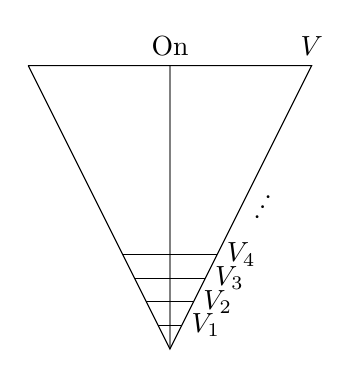
\begin{tikzpicture}[scale = 0.6]
\draw[gray] (0,0) -- (0,6);
\draw (-3,6) -- (0,0) -- (3,6) -- (-3,6);
\draw (-0.25,0.5) -- (0.25,0.5);
\draw (-0.5,1) -- (0.5,1);
\draw (-0.75,1.5) -- (0.75,1.5);
\draw (-1,2) -- (1,2);
\node[above] at (0,6) {$\Ordinals$};
\node[right] at (0.25,0.5) {$V_1$};
\node[right] at (0.5,1) {$V_2$};
\node[right] at (0.75,1.5) {$V_3$};
\node[right] at (1,2) {$V_4$};
\node[right,rotate=-30] at (1.8,3.3) {$\vdots$};
\node[above] at (3,6) {$V$};
\end{tikzpicture}
\]



\section{ハイティング代数とブール代数}

半順序集合$L$であって任意の2元が最小上界,最大下界を持つようなものを{\bfseries 束}という.
2元$a, b$の最小上界を$a \lor b$, $a, b$の最大下界を$a \land b$と書く.最大元と最小元のある束を{\bfseries 有界束}という.最大元を$1$,最小元を$0$で書く.
束が{\bfseries 完備}であるとは任意の部分集合が最小上界と最大下界を持つときを言う.
元が添え字づけられた部分集合$\{a_i\}_{i \in I}$の最小上界を$\bigvee_{i \in I} a_i$, 最大下界を$\bigwedge_{i \in I} a_i$と書く.

束が{\bfseries 分配束}であるとは任意の元$x, y, z$に対して
\[
x \land (y \lor z) = (x \land y) \lor (x \land z),\hspace{0.2cm}
x \lor (y \land z) = (x \lor y) \land (x \lor z)
\]
をみたすときをいう.


有界束$H$が{\bfseries ハイティング代数}であるとは,任意の2元$x, y \in H$に対して$\{ z \in H : z \land x \le y \}$が最大元を持つときを言う.この最大元を$(x \Rightarrow y)$で書く.これは次で特徴付けられる:
\[
z \le (x \Rightarrow y) \iff z \land x \le y.
\]
$x \in H$に対し$x^* = (x \Rightarrow 0)$と定義し,$x$の{\bfseries 疑補元}という.
ハイティング代数は常に分配束である (少し計算が必要).

ハイティング代数の最も重要な例は位相空間$X$の開集合系$\mathcal{O}(X)$で通常の包含で順序を入れたものであり,これは完備ハイティング代数である.
このハイティング代数において,最小元は$\emptyset$, 最大元は$X$であり,演算は次で計算できる:
\begin{align*}
\bigvee_{i \in I} U_i &= \bigcup_{i \in I} U_i, \\
\bigwedge_{i \in I} U_i &= \intr \bigcap_{i \in I} U_i, \\
(U \Rightarrow V) &= \intr (U^c \cup V), \\
U^* &= \intr (U^c).
\end{align*}
ただしここで$\intr$は内部を表す.

$L$を有界束とする.
$a \in L$の補元とは$b \in L$であって,$a \land b = 0, a \lor b = 1$をみたすもののことである.
ハイティング代数$H$で疑補元は必ずしも補元ではない.すべての疑補元が補元である,すなわちすべての$x \in H$について$x \lor x^* = 1$を満たすハイティング代数$H$を{\bfseries ブール代数}という.
ブール代数では$(x \Rightarrow y) = x^* \lor y$であることが容易に示せる.ブール代数であることは任意の元が補元を持つ分配束であることと同値である.

ブール代数の重要な例は位相空間$X$の正則開集合全体の集合$\RO(X)$に通常の包含で順序を入れたものである:
\[
\RO(X) = \{ U \subset X : \text{$U$は正則開集合} \}
\]
ここで$X$の部分集合$U$が正則開集合とは$\intr \cl U = U$を満たすことをいう.
ただし$\cl$は閉包.これは完備ブール代数であり演算は次で計算できる:
\begin{align*}
\bigvee_{i \in I} U_i &= \intr \cl \bigcup_{i \in I} U_i, \\
\bigwedge_{i \in I} U_i &= \intr \cl  \bigcap_{i \in I} U_i, \\
U^* &= \intr (U^c).
\end{align*}

\section{ブール代数値モデル}

\begin{defi}
$B$を完備ブール代数とする.{\bfseries $B$名称}の全体のクラス$V^B$を次で定義する:
\begin{align*}
V^B_0 &= \emptyset \\
V^B_{\alpha + 1} &= \{ \dot{x} : \Func(\dot{x}) \land \dom(\dot{x}) \subset V^B_\alpha \land \range(\dot{x}) \subset B \} \\
V^B_{\gamma} &= \bigcup_{\alpha < \gamma} V^B_\alpha \ \text{($\gamma$は極限順序数)} \\
V^B &= \bigcup_{\alpha \in \Ordinals} V^B_\alpha
\end{align*}
\end{defi}

$B$名称は直観的には所属関係に確率が付随した集合である.
$\dot{x}, \dot{y}$という$B$名称に対して$\dot{y}(\dot{x})$という$B$の元は$\dot{x}$が$\dot{y}$の中に入っている確率と思ってよい.
以下の例でそれを実感してほしい.

\begin{exm}
$B$を位相空間$[0, 1]$の正則開集合全体のなす完備ブール代数とする.
\[
\dot{\emptyset} = \emptyset
\]
はB名称である.
また,
\begin{align*}
\dom(\dot{x}) &= \{\dot{\emptyset}\} \\
\dot{x}(\dot{\emptyset}) &= [0, 0.5)
\end{align*}
なる$\dot{x}$もB名称である.
\begin{align*}
\dom(\dot{y}) &= \{\dot{x}\} \\
\dot{y}(\dot{x}) &= (0.4, 0.6)
\end{align*}
なる$\dot{y}$もB名称である.
以下で論理式$\varphi$の成り立つ確率$\truth{\varphi}$を定義するが,その下で
\begin{align*}
\truth{\dot{\emptyset} = \emptyset} &= [0, 1] \\
\truth{\dot{x} = \{\emptyset\}} &= [0, 0.5) \\
\truth{\dot{x} = \emptyset} &= (0.5, 1] \\
\truth{\dot{y} = \{\{\emptyset\}\}} &= (0.4, 0.5) \\
\truth{\dot{y} = \{\emptyset\}} &= (0.5, 0.6) \\
\truth{\dot{y} = \emptyset} &= [0, 0.4) \cup (0.6, 1] \end{align*}
となる.
\[
\begin{tikzpicture}
\draw (0,0) -- (0,3);

\draw [fill=black] (0,0) circle (0.05) node[above right] {$\dot{\emptyset}$};
\draw [fill=black] (0,1.5) circle (0.05) node[above right] {$\dot{x}$};
\draw [fill=black] (0,3) circle (0.05) node[above right] {$\dot{y}$};

\draw (-1.5,0.6) -- (-0.5,0.6);
\draw (-1.5,0.6) -- (-1.4,0.7) --  (-1.1,0.7) -- (-1,0.6);

\draw (-1.5,2.1) -- (-0.5,2.1);
\draw (-1.1,2.1) -- (-1.05,2.2) -- (-0.95,2.2) -- (-0.9,2.1);

\end{tikzpicture}
\]
\end{exm}

\begin{defi}\label{atomicfml}
$\dot{x}, \dot{y} \in V^B$に対して
\begin{align*}
\truth{\dot{x} \in \dot{y}} &= \bigvee_{\dot{z} \in \dom \dot{y}} (\dot{y}(\dot{z}) \land \truth{\dot{x} = \dot{z}}) \\
\truth{\dot{x} = \dot{y}} &= \bigwedge_{\dot{z} \in \dom \dot{y}} (\dot{y}(\dot{z}) \Rightarrow \truth{\dot{z} \in \dot{x}}) \land \bigwedge_{\dot{z} \in \dom \dot{x}} (\dot{x}(\dot{z}) \Rightarrow \truth{\dot{z} \in \dot{y}})
\end{align*}
と定める.
\end{defi}
$\truth{\cdot \in \cdot}$の定義に$\truth{\cdot = \cdot}$を使って,
$\truth{\cdot = \cdot}$の定義に$\truth{\cdot \in \cdot}$を使っているが,これは再帰的定義の一種である.定義に使っている名称のランクがある意味で下がっているのでこの再帰が正当化される.

$B$名称すべてを定数記号に持つ言語を考え,この言語の論理式を{\bfseries $B$論理式}という.

\begin{defi}
$B$閉論理式$\varphi$に対して$\varphi$の真理値($\varphi$の成り立つ確率)$\truth{\varphi}$を次で定義:
\begin{enumerate}
    \item $\varphi$が原子論理式の場合は定義\ref{atomicfml}の通り.
    \item $\truth{\varphi \land \psi} = \truth{\varphi} \land \truth{\psi}$
    \item $\truth{\varphi \lor \psi} = \truth{\varphi} \lor \truth{\psi}$
    \item $\truth{\neg \varphi} = \truth{\varphi}^*$
    \item $\truth{\varphi \to \psi} = (\truth{\varphi} \Rightarrow \truth{\psi})$
    \item $\truth{\forall x\ \varphi} = \bigwedge_{\dot{x} \in V^B} \truth{\varphi(\dot{x})}$
    \item $\truth{\exists x\ \varphi} = \bigvee_{\dot{x} \in V^B} \truth{\varphi(\dot{x})}$
\end{enumerate}
\end{defi}

$\truth{\varphi} = 1$となるとき$\varphi$は$V^B$で正しいという.

\begin{thm}
$B$を完備ブール代数とする.ZFCのすべての公理は$V^B$で正しい.また$V^B$で正しい論理式全体は一階述語論理の推論規則で閉じている.
\end{thm}

この定理を部分的に証明する.
まず,命題論理の公理,たとえば$(\varphi \land \psi)\to \varphi$などが正しいことは明らかであろう.

一階述語論理の公理の中から等号の反射性$\forall x\ (x = x)$をとって証明してみよう.

\begin{lem}
等号の反射性$\forall x\ (x = x)$は$V^B$で正しい.
\end{lem}
\begin{proof}
$\dot{x}$のランクに関する帰納法で示す.$\dot{x} \in V^B$とする.
\begin{align*}
\truth{\dot{x} = \dot{x}} &= \bigwedge_{\dot{z} \in \dom \dot{x}} (\dot{x}(\dot{z}) \Rightarrow \truth{\dot{z} \in \dot{x}}) \\
&= \bigwedge_{\dot{z} \in \dom \dot{x}} (\dot{x}(\dot{z}) \Rightarrow \bigvee_{\dot{w} \in \dom \dot{x}} (\dot{x}(\dot{w}) \land \truth{\dot{z} = \dot{w}}))
\end{align*}
であるが,$\dot{z} \in \dom \dot{x}$について
\[
\bigvee_{\dot{w} \in \dom \dot{x}} (\dot{x}(\dot{w}) \land \truth{\dot{z} = \dot{w}}) \ge \dot{x}(\dot{z}) \land \truth{\dot{z} = \dot{z}} = \dot{x}(\dot{z}).
\]
である.最後の等号は$\dot{z}$は$\dot{x}$よりランクが下がっているので帰納法の仮定が使えて$\truth{\dot{z} = \dot{z}} = 1$となることを使った.
よって
\begin{align*}
\truth{\dot{x} = \dot{x}} &= \bigwedge_{\dot{z} \in \dom \dot{x}} (\dot{x}(\dot{z}) \Rightarrow \bigvee_{\dot{w} \in \dom \dot{x}} (\dot{x}(\dot{w}) \land \truth{\dot{z} = \dot{w}})) \\
&\ge \bigwedge_{\dot{z} \in \dom \dot{x}} (\dot{x}(\dot{z}) \Rightarrow \dot{x}(\dot{z})) \\
&\ge \bigwedge_{\dot{z} \in \dom \dot{x}} 1 \\
&= 1
\end{align*}
となる.
\end{proof}

上の証明から容易に,任意の名称$\dot{x}, \dot{y}$について
\[
\dot{y}(\dot{x}) \le \truth{\dot{x} \in \dot{y}} 
\]
が分かる.

他の等号公理$\forall x, y, z\ ((x = y \land y = z) \to x = z)$や$\forall x, y, z\ ((x = y \land y \in z) \to x \in z)$なども示すことができるが,証明は省略する.

以上より一階述語論理の公理はすべて$V^B$で正しいことが分かった.また,推論規則が正しい論理式から正しい論理式を導くことも容易に分かる.

次の命題はあとで使う.
\begin{prop}
\begin{enumerate}
    \item $\truth{\exists x \in \dot{y}\ \varphi(x)} = \bigvee_{\dot{x} \in \dom \dot{y}} (\dot{y}(\dot{x}) \land \truth{\varphi(\dot{x})})$
    \item $\truth{\forall x \in \dot{y}\ \varphi(x)} = \bigwedge_{\dot{x} \in \dom \dot{y}} (\dot{y}(\dot{x}) \Rightarrow \truth{\varphi(\dot{x})})$
\end{enumerate}
\end{prop}


ここからZFCの公理の中からいくつか選んで$V^B$で正しいことを示そう.具体的には対公理,和集合公理,無限公理が正しいことを示す.

\begin{lem}
対公理は$V^B$で正しい.
\end{lem}
\begin{proof}
示すべきは
\[
\truth{\forall a, b\ \exists C\ \forall x\ ((x = a \lor x = b) \leftrightarrow x \in C)} = 1
\]
である.そこで$\dot{a}, \dot{b} \in V^B$を任意にとる.このとき
\[
\truth{\exists C\ \forall x\ ((x = \dot{a} \lor x = \dot{b}) \leftrightarrow x \in C)} = 1
\]
を示す.
\[
\dot{C} = \{ (\dot{a}, 1), (\dot{b}, 1) \}
\]
とおく.このとき
\[
\truth{\forall x\ ((x = \dot{a} \lor x = \dot{b}) \leftrightarrow x \in \dot{C})} = 1
\]
を示せば十分である.そこで$\dot{x} \in V^B$を任意にとる.すると
\begin{align*}
\truth{\dot{x} \in \dot{C}} &= \bigvee_{\dot{y} \in \dom \dot{C}} (\dot{C}(\dot{y}) \land \truth{\dot{x} = \dot{y}}) \\
&= (\dot{C}(\dot{a}) \land \truth{\dot{x} = \dot{a}}) \lor (\dot{C}(\dot{b}) \land \truth{\dot{x} = \dot{b}}) \\
&= \truth{\dot{x} = \dot{a}} \lor \truth{\dot{x} = \dot{b}}
\end{align*}
となるのでよい.
\end{proof}

この証明で分かるように,与えられた名称$\dot{a}, \dot{b}$に対して
\[
\{\dot{a}, \dot{b}\}^B = \{ (\dot{a}, 1), (\dot{b}, 1) \}
\]
とおけばこれが対の名称になっている.

\begin{lem}
和集合公理は$V^B$で正しい.
\end{lem}
\begin{proof}
示すべきは
\[
\truth{\forall \mathcal{A}\ \exists B\ \forall x\ (\exists Y\ (x \in Y \land Y \in \mathcal{A}) \leftrightarrow x \in B)} = 1
\]
である.
そこで$\dot{\mathcal{A}} \in V^B$を任意にとる.名称$\dot{B}$を次で定める:
\begin{align*}
\dom \dot{B} &= \bigcup_{\dot{X} \in \dom \dot{\mathcal{A}}} \dom \dot{X}, \\
\dot{B}(\dot{x}) &= \truth{\exists Y\ (\dot{x} \in Y \land Y \in \dot{\mathcal{A}})}\ \text{ (for each $\dot{x} \in \dom \dot{B})$}.
\end{align*}
これが求めるべき名称になっている:
\[
\truth{\forall x\ (\exists Y\ (x \in Y \land Y \in \dot{\mathcal{A}}) \leftrightarrow x \in \dot{B})} = 1.
\]
このことの確認は省略する.

イメージは次の通りである.$\dot{\mathcal{A}}$の子供の子供を集めてきて,それらを適切な確率で子供に持つ名称$\dot{B}$を作ったのである.
\[
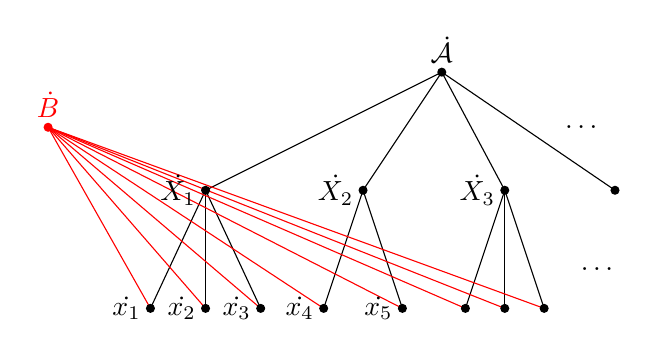
\begin{tikzpicture}
\draw (0,0) -- (-3,-1.5);
\draw (0,0) -- (-1,-1.5);
\draw (0,0) -- (0.8,-1.5);
\draw (0,0) -- (2.2,-1.5);

\draw (-3,-1.5) -- (-3.7,-3);
\draw (-3,-1.5) -- (-3,-3);
\draw (-3,-1.5) -- (-2.3,-3);

\draw (-1,-1.5) -- (-1.5,-3);
\draw (-1,-1.5) -- (-0.5,-3);

\draw (0.8,-1.5) -- (0.3,-3);
\draw (0.8,-1.5) -- (0.8,-3);
\draw (0.8,-1.5) -- (1.3,-3);

\draw [red,fill=red] (-5,-0.7) circle (0.05) node[above] {$\dot{B}$};
\draw [red] (-5,-0.7) -- (-3.7,-3);
\draw [red] (-5,-0.7) -- (-3,-3);
\draw [red] (-5,-0.7) -- (-2.3,-3);
\draw [red] (-5,-0.7) -- (-1.5,-3);
\draw [red] (-5,-0.7) -- (-0.5,-3);
\draw [red] (-5,-0.7) -- (0.3,-3);
\draw [red] (-5,-0.7) -- (0.8,-3);
\draw [red] (-5,-0.7) -- (1.3,-3);

\draw [fill=black] (0,0) circle (0.05) node[above] {$\dot{\mathcal{A}}$};
\draw [fill=black] (-3,-1.5) circle (0.05) node[left] {$\dot{X_1}$};
\draw [fill=black] (-1,-1.5) circle (0.05) node[left] {$\dot{X_2}$};
\draw [fill=black] (0.8,-1.5) circle (0.05) node[left] {$\dot{X_3}$};
\draw [fill=black] (2.2,-1.5) circle (0.05);

\draw [fill=black] (-3.7,-3) circle (0.05) node[left] {$\dot{x_1}$};
\draw [fill=black] (-3,-3) circle (0.05) node[left] {$\dot{x_2}$};
\draw [fill=black] (-2.3,-3) circle (0.05) node[left] {$\dot{x_3}$};
\draw [fill=black] (-1.5,-3) circle (0.05) node[left] {$\dot{x_4}$};
\draw [fill=black] (-0.5,-3) circle (0.05) node[left] {$\dot{x_5}$};
\draw [fill=black] (0.3,-3) circle (0.05);
\draw [fill=black] (0.8,-3) circle (0.05);
\draw [fill=black] (1.3,-3) circle (0.05);

\node at (1.8,-0.7) {$\dots$};
\node at (2,-2.5) {$\dots$};
\end{tikzpicture}
\]


%まず,
%\begin{align*}
%\truth{\forall x \in B\ \exists Y\ (x \in Y \land Y \in \dot{\mathcal{A}})}
%&= \bigwedge_{\dot{x} \in \dom \dot{B}} (\dot{B}(\dot{x}) \Rightarrow \truth{\exists Y\ (\dot{x} \in Y \land Y \in \dot{\mathcal{A}})}) \\
%&= \bigwedge_{\dot{x} \in \dom \dot{B}} (\truth{\exists Y\ (\dot{x} \in Y \land Y \in \dot{\mathcal{A}})} \Rightarrow \truth{\exists Y\ (\dot{x} \in Y \land Y \in \dot{\mathcal{A}})}) \\
%&= \bigwedge_{\dot{x} \in \dom \dot{B}} 1 \\
%&= 1
%\end{align*}
%である.
%$\dot{x} \in V^B$を任意にとる.
%このとき
%\begin{align*}
%\truth{\exists Y \in \dot{\mathcal{A}}\ (\dot{x} \in Y)} &= \bigvee_{\dot{Y} \in \dom \dot{\mathcal{A}}} (\dot{\mathcal{A}}(\dot{Y}) \land \truth{\dot{x} \in \dot{Y}}) \\
%&= \bigvee_{\dot{Y} \in \dom \dot{\mathcal{A}}} (\dot{\mathcal{A}}(\dot{Y}) \land \bigvee_{\dot{y} \in \dom \dot{Y}} (\dot{Y}(\dot{y}) \land \truth{\dot{x} = \dot{y}})) \\
%&= \bigvee_{\dot{Y} \in \dom \dot{\mathcal{A}}}  \bigvee_{\dot{y} \in \dom \dot{Y}} ((\dot{\mathcal{A}}(\dot{Y}) \land \dot{Y}(\dot{y})) \land \truth{\dot{x} = \dot{y}})
%\end{align*}
%である.今,
%\[
%\dot{\mathcal{A}}(\dot{Y}) \land \dot{Y}(\dot{y}) \le \truth{\dot{y} \in \dot{B}}
%\]
%であるので,
%\begin{align*}
%\truth{\exists Y \in \dot{\mathcal{A}}\ (\dot{x} \in Y)} &= \bigvee_{\dot{Y} \in \dom \dot{\mathcal{A}}}  \bigvee_{\dot{y} \in \dom \dot{Y}} ((\dot{\mathcal{A}}(\dot{Y}) \land \dot{Y}(\dot{y})) \land \truth{\dot{x} = \dot{y}}) \\
%&\le \bigvee_{\dot{Y} \in \dom \dot{\mathcal{A}}}  \bigvee_{\dot{y} \in \dom \dot{Y}} \truth{\dot{y} \in \dot{B}} \land \truth{\dot{x} = \dot{y}}) \\
%&\le \bigvee_{\dot{Y} \in \dom \dot{\mathcal{A}}}  \bigvee_{\dot{y} \in \dom \dot{Y}} \truth{\dot{x} \in \dot{B}} \\
%&\le \truth{\dot{x} \in \dot{B}}.
%\end{align*}
%これでOK.

\end{proof}

無限公理を確かめるために,まずチェック名称というものを定める.

\begin{defi}
集合$x$に対して
\[
\check{x} = \{ (\check{y}, 1) : y \in x \}
\]
と定める.これはランク再帰である.
\end{defi}

\begin{defi}
すべての量化記号$\forall, \exists$の出現が$\forall x \in y$や$\exists x \in y$のような形になっている論理式を{\bfseries $\Delta_0$論理式}と呼ぶ.
\end{defi}

\begin{prop}
$\varphi(x_1, \dots, x_n)$を$\Delta_0$論理式とし,$u_1, \dots, u_n$を集合とするとき,
\[
\varphi(u_1, \dots, u_n) \iff \truth{\varphi(\check{u_1}, \dots, \check{u_n})} = 1
\]
である.
\end{prop}
証明は省略する.

さて,無限公理
\[
\exists A\ (\emptyset \in A \land \forall x \in A\ (x \cup \{x\} \in A))
\]
の$\exists A$の中身
\[
\emptyset \in A \land \forall x \in A\ (x \cup \{x\} \in A)
\]
は$\Delta_0$論理式で書ける.
したがって,$\omega$のチェック名称$\check{\omega}$について
\[
\truth{\emptyset \in \check{\omega} \land \forall x \in \check{\omega}\ (x \cup \{x\} \in \check{\omega})} = 1
\]
が成り立つ.これで無限公理が正しいことが示せた.

\section{ブール代数値モデルの応用}

\subsection{コーエン強制$\RO(2^\omega)$}

完備ブール代数$B = \RO(2^\omega)$を考える.
ただし$2^\omega$には$2$を離散空間としたときの直積位相を入れている.

$\dot{g} \in V^B$という名称を$\dom \dot{g} = \dom \check{\omega}$かつ各$n \in \omega$に対して
\[
\dot{g}(\check{n}) = \{ f \in 2^\omega : f(n) = 1 \} \in \RO(2^\omega)
\]
で定める.

\[
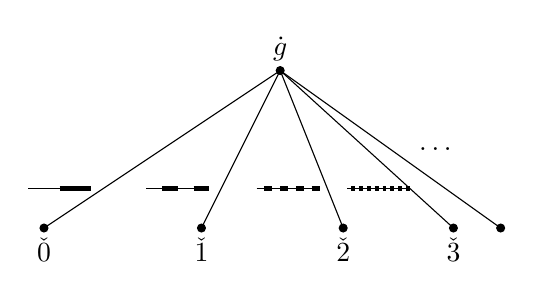
\begin{tikzpicture}
\draw (0,0) -- (-3,-2);
\draw (0,0) -- (-1,-2);
\draw (0,0) -- (0.8,-2);
\draw (0,0) -- (2.2,-2);
\draw (0,0) -- (2.8,-2);

\draw [fill=black] (0,0) circle (0.05) node[above] {$\dot{g}$};
\draw [fill=black] (-3,-2) circle (0.05) node[below] {$\check{0}$};
\draw [fill=black] (-1,-2) circle (0.05) node[below] {$\check{1}$};
\draw [fill=black] (0.8,-2) circle (0.05) node[below] {$\check{2}$};
\draw [fill=black] (2.2,-2) circle (0.05) node[below] {$\check{3}$};
\draw [fill=black] (2.8,-2) circle (0.05);
\node at (2,-1) {$\dots$};

\begin{scope}[shift={(-3.2,-1.5)}, scale=0.8]
\draw (0,0) -- (1,0);
\draw[line width=0.7mm] (0.5,0) -- (1,0);
\end{scope}

\begin{scope}[shift={(-1.7,-1.5)}, scale=0.8]
\draw (0,0) -- (1,0);
\draw[line width=0.7mm] (0.25,0) -- (0.5,0);
\draw[line width=0.7mm] (0.75,0) -- (1,0);
\end{scope}

\begin{scope}[shift={(-0.3,-1.5)}, scale=0.8]
\draw (0,0) -- (1,0);
\draw[line width=0.7mm] (0.125,0) -- (0.25,0);
\draw[line width=0.7mm] (0.375,0) -- (0.5,0);
\draw[line width=0.7mm] (0.625,0) -- (0.75,0);
\draw[line width=0.7mm] (0.875,0) -- (1,0);
\end{scope}

\begin{scope}[shift={(0.85,-1.5)}, scale=0.8]
\draw (0,0) -- (1,0);
\draw[line width=0.7mm] (0.0625,0) -- (0.125,0);
\draw[line width=0.7mm] (0.1875,0) -- (0.25,0);
\draw[line width=0.7mm] (0.3125,0) -- (0.375,0);
\draw[line width=0.7mm] (0.4375,0) -- (0.5,0);
\draw[line width=0.7mm] (0.5625,0) -- (0.625,0);
\draw[line width=0.7mm] (0.6875,0) -- (0.75,0);
\draw[line width=0.7mm] (0.8125,0) -- (0.875,0);
\draw[line width=0.7mm] (0.9375,0) -- (1.0,0);
\end{scope}
\end{tikzpicture}
\]


\[
\truth{\dot{g} \in \PP(\omega)} = 1
\]
は明らか.

さて,どんな$x \in \PP(\omega)$についても$\truth{\dot{g} = \check{x}} = 0$なことを示そう.
\begin{align*}
\truth{\dot{g} = \check{x}} &= \bigwedge_{n \in \omega} (\dot{g}(\check{n}) \Leftrightarrow \truth{\check{n} \in \check{x}}) \\
&= \intr \cl \bigcap_{n \in \omega} \{ f \in 2^\omega : f(n) = 1 \iff n \in x \} \\
&= \intr \cl \{\chi_x\} = \emptyset
\end{align*}
よりよい.ここに最後の$\chi_x$は$x$の特徴関数である.

したがって,
\[
1 = \truth{\dot{g} \in \PP(\omega)} \land \truth{\dot{g} \not \in  (\PP(\omega))^{\vee}} \le \truth{\PP(\omega) \ne (\PP(\omega))^{\vee}}
\]
である.

これは$V^B$には$V$にない新しい$\omega$の部分集合が付け加わっていることを意味する.

\subsection{コーエン強制$\RO(2^{\omega \times \omega_2})$}

完備ブール代数$B = \RO(2^{\omega \times \omega_2})$を考える.
これも離散空間の直積である.

各$\alpha < \omega_2$に対して$\dot{g}_\alpha \in V^B$という名称を$\dom \dot{g}_\alpha = \dom \check{\omega}$かつ各$n \in \omega$に対して
\[
\dot{g}_\alpha(\check{n}) = \{ f \in 2^{\omega \times \omega_2} : f(n, \alpha) = 1 \} \in \RO(2^{\omega \times \omega_2})
\]
で定める.

どんな$\alpha, \beta < \omega_2, \alpha \ne \beta$についても$\truth{\dot{g}_\alpha = \dot{g}_\beta} = 0$であることを確かめよう.
\begin{align*}
\truth{\dot{g}_\alpha = \dot{g}_\beta} &= \intr \cl \{ f \in 2^{\omega \times \omega_2} : \forall n \in \omega\ f(n, \alpha) = f(n, \beta) \} \\
 &= \intr \{ f \in 2^{\omega \times \omega_2} : \forall n \in \omega\ f(n, \alpha) = f(n, \beta) \}
\end{align*}
である.最右辺の$\intr$の中身
\[
F = \{ f \in 2^{\omega \times \omega_2} : \forall n \in \omega\ f(n, \alpha) = f(n, \beta) \}
\]
が実際は内点を持たないことを言えばよい.内点を持つとすると位相の入れ方より有限な関数$p$があって$\dom p \subset \omega \times \omega_2, \range p \subset 2$であり,$N_p = \{ f : p \subset f \}$が$F$の部分集合である.

$n \in \omega$であって,どんな$\xi < \omega_2$についても$(n, \xi) \not \in \dom p$なものをとる ($p$の有限性よりとれる).
そして
\[
p' = p \cup \{ ((n, \alpha), 0), ((n, \beta), 1) \}
\]
とおく.すると
\[
N_{p'} \subset N_p \subset F
\]
だが,
$N_{p'}$の中の一点$f$ (空でないのでとれる)を考えると
\[
f(n, \alpha) = 0 \land f(n, \beta) = 1 \land f(n, \alpha) = f(n, \beta)
\]
となって矛盾.

さて
\[
\dot{f} = \{ ((\check{\alpha}, \dot{g}_\alpha)^B, 1) : \alpha < \omega_2 \}
\]
とおく.ただし,名称$\dot{x}, \dot{y}$に対して
\begin{align*}
\{\dot{x}, \dot{y}\}^B &= \{ (\dot{x}, 1), (\dot{y}, 1) \} \\
(\dot{x}, \dot{y})^B &= \{\{\dot{x}, \dot{x}\}^B, \{\dot{x}, \dot{y}\}^B\}^B
\end{align*}
である.
このとき
\[
\truthtext{$\dot{f}$は$\check{\omega_2}$から$2^\omega$への写像} = 1
\]
であるし,しかも,上の議論から
\[
\truthtext{$\dot{f}$は単射} = 1
\]
である.したがって,
\[
\truth{2^{\aleph_0} \ge |\check{\omega_2}|} = 1
\]
である.一見,これで連続体仮説の否定の無矛盾性が示せたように思えるが,まだである.というのは
\[
\truth{|\check{\omega_2}| = \omega_2} = 1
\]
である保証はないからだ.実際,一般の完備ブール代数では基数は保存されない.しかし,cccと呼ばれる性質を満たすブール代数では基数は保存され,しかも今考えているブール代数$\RO(2^{\omega \times \omega_2})$はうれしいことにcccを持ってくれるのである.以下このことを概説しよう.

\subsubsection{cccと基数保存}

\begin{defi}
位相空間$X$が{\bfseries ccc (countable chain condition)}を満たすとは$X$の非空開集合の族で互いに交わらないものは必ず可算であることを言う.

ブール代数$B$の部分集合$A \subset B \setminus \{0\}$が{\bfseries 反鎖}であるとは$A$の任意の異なる2元$a, b$が$a \land b = 0$を満たすことを言う.

ブール代数$B$が{\bfseries ccc}を満たすとは,どんな$B$の反鎖も可算となることをいう.
\end{defi}

反鎖は次のように互いに交わらない部分集合の族でイメージすればよいだろう.
\[
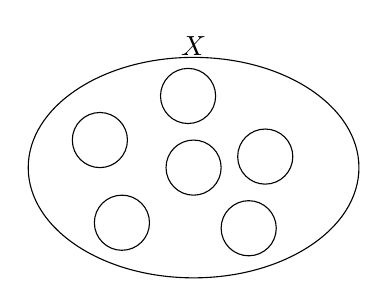
\begin{tikzpicture}[scale=0.7]
\node at (0,2.2) {$X$};
\draw (0,0) ellipse (3 and 2);
\draw (0,0) circle (0.5);
\draw (1.3,0.2) circle (0.5);
\draw (-1.7,0.5) circle (0.5);
\draw (-0.1,1.3) circle (0.5);
\draw (-1.3,-1) circle (0.5);
\draw (1,-1.1) circle (0.5);
\end{tikzpicture}
\]


どんな集合$I$についても直積空間$2^I$はcccを持つことが知られている.これはデルタシステム補題という補題を使って証明される.
また,位相空間$X$がcccを満たすならば,正則開集合の代数$\RO(X)$がcccを満たすことは明らか.
よって上で考えていたブール代数$\RO(2^{\omega \times \omega_2})$はcccを満たす.

cccな完備ブール代数のよいところは基数を保存することである.すなわち,次が成り立つ.

\begin{thm}
$B$をcccを満たす完備ブール代数とする.
このとき任意の$\kappa$について
\[
\text{$\kappa$が基数} \iff \truthtext{$\check{\kappa}$が基数} = 1.
\]
\end{thm}
\begin{proof}
まず,$\truthtext{$\check{\alpha}$が基数} = 1$ならば$\alpha$が基数であることは$B$がcccでなくても常に言える.
なぜならば,まず$\alpha$が順序数であることは$\Delta_0$で書ける.$\in$で全順序付けされていて推移的集合であると書けばいいからだ (正則性公理よりwell-foundednessは書く必要がない).
そして順序数$\alpha$が基数であるという条件は,
\[
\neg \exists f\ \exists \beta < \alpha\ (\textwospace{$f : \beta \to \alpha$全射}) 
\]
と書けるが$f : \beta \to \alpha$全射の部分は$\Delta_0$である.

もし$V$で$\alpha$が基数でなければ,上のような$f$と$\beta < \alpha$をとれるが,そのチェック名称を考えれば,
\[
\truthtext{$\check{\beta} < \check{\alpha} \land \check{f} : \check{\beta} \to \check{\alpha}$全射} = 1
\]
である.よって,
\[
\truth{\exists f\ \exists \beta < \check{\alpha}\ (\textwospace{$f : \beta \to \check{\alpha}$全射})} = 1
\]
なので$\truthtext{$\check{\alpha}$は基数} = 0$である.
したがって,$\truthtext{$\check{\alpha}$が基数} = 1$ならば$\alpha$が基数である.

さて,$\kappa$が基数とする.
このとき$\truthtext{$\check{\kappa}$が基数} = 1$を示す.
$\kappa$が$\omega$以下の場合は$\truth{\check{\omega} = \omega} = 1$より容易に従う.そこで$\kappa$を非可算とする.

$\truthtext{$\check{\kappa}$が基数} = 1$を示すには任意に与えられた$\dot{f} \in V^B$と$\beta < \kappa$に対して
\[
\truthtext{$\dot{f} : \check{\beta} \to \check{\kappa}$全射} = 0
\]
を示せばよい.$a = \truthtext{$\dot{f} : \check{\beta} \to \check{\kappa}$全射}$とおき,$a \ne 0$と仮定する.
すると
\[
0 \ne a \le \bigwedge_{\eta < \kappa} \bigvee_{\xi < \beta} (\truth{\dot{f}(\check{\xi}) = \check{\eta}} \land a)
\]
である.よって各$\eta < \kappa$について$\xi_\eta < \beta$が存在して
\[
\truth{\dot{f}(\check{\xi_\eta}) = \check{\eta}} \land a \ne 0
\]
が従う.
$\kappa$が非可算基数で,$\beta < \kappa$なので鳩の巣原理よりある$\gamma < \beta$が存在して
\[
X = \{ \eta < \kappa : \xi_\eta = \gamma \}
\]
が非可算となる.したがって,
\[
\{ \truth{\dot{f}(\check{\gamma}) = \check{\eta}} \land a : \eta \in X \}
\]
が非可算な反鎖となり,これは$B$がcccなことに反する.
\end{proof}

上の$\RO(2^{\omega \times \omega_2})$に関する議論とこの定理とを合わせると次を得る.

\begin{thm}
$B = \RO(2^{\omega \times \omega_2})$について$V^B$で
\[
2^{\aleph_0} \ge \aleph_2
\]
が正しい.
特に,ZFCが無矛盾ならばそれに$2^{\aleph_0} \ge \aleph_2$を足したものも無矛盾である.
\end{thm}

\section{ハイティング代数値モデルとその応用}
\label{sec:heyting}

ここからは直観主義論理のモデルを作るが,その議論は依然としてZFCの中で行う.
今までの議論の完備ブール代数を完備ハイティング代数にそのまま置き換えるだけでハイティング代数値モデルができる.
ブール代数値モデルではZFCのモデルができたが,ハイティング代数ではIZFのモデルができる.

IZFはベースとする論理を直観主義論理にして,集合論的公理として選択公理以外の公理1~8を入れたものである.

\begin{thm}
$H$を完備ハイティング代数とする.IZFのすべての公理は$V^H$で正しい.また$V^H$で正しい論理式全体は直観主義の一階述語論理の推論規則で閉じている.
\end{thm}

\subsection{無限だがデデキント有限な$\omega$の部分集合の存在}\label{infbutdedfin}

ハイティング代数値モデルの一つの例を見てみよう.

$\omega$に上に閉じた集合を開集合とする位相を入れる.
この位相空間の開集合系がなる完備ハイティング代数を$H$とする.
すなわち
\[
H = \{ O_n : n \in \omega \} \cup \{\emptyset\}
\]
で
\[
O_n = \{ m \in \omega : m \ge n \}
\]
である.
$K \in V^H$を次で定義する.
\[ \dom \dot{K} = \dom \check{\omega} \]
で,各$n \in \omega$について
\[ \dot{K}(\check{n}) = O_n \]
である.

このとき次のハイティング代数値を計算してみよう.

\begin{align*}
\truth{\forall x \in \omega\ \exists y \in \dot{K}\ x < y} &= \bigwedge_{x \in \omega} \bigvee_{y \in \omega} (\truth{\check{y} \in \dot{K}} \land \truth{\check{x} < \check{y}}) \\
 &= \bigwedge_{x \in \omega} \bigvee_{y \ge x} \truth{\check{y} \in \dot{K}} \\
 &= \intr \bigcap_{x \in \omega} \bigcup_{y \ge x} O_y \\
 &= \intr \bigcap_{x \in \omega} O_x \\
 &= \intr \emptyset \\
 &= \emptyset
\end{align*}

\begin{align*}
\truth{\exists x \in \omega\ \forall y \in \dot{K}\ y \le x} &= \bigvee_{x \in \omega} \bigwedge_{y \in \omega} (\truth{\check{y} \in \dot{K}} \Rightarrow \truth{\check{y} \le \check{x}}) \\
 &= \bigvee_{x \in \omega} \bigwedge_{y > x} \truth{\check{y} \in \dot{K}}^* \\
 &= \bigcup_{x \in \omega} \intr (\bigcap_{y > x} \intr(\omega - O_y)) \\
 &= \emptyset
\end{align*}

最初の例は「どんな自然数に対してもそれより大きい$K$の元が存在する」が確率$0$,次の例は「ある自然数一個ですべての$K$の元を上から抑えられる」が確率$0$なことを言っている.
奇妙に見えるが,これは$V^H$で$\dot{K}$が無限だがデデキント有限なことを意味している.

ここで$\omega$の部分集合$A$が有限とはある自然数$n$と$n$から$A$への全単射が存在することとする.\footnote{正確には「ある自然数$n$と$n$から$A$への全単射が存在すること」はstrictly finiteという条件である.しかし$\omega$の部分集合については有限とstrictly finiteは同値なのでこのように定義した.}また,$A$がデデキント無限とは,$f: \omega \to A$単射が存在することとし,デデキント有限とはデデキント無限でないこととする.
次が言える.
\begin{align}
\text{$A$がデデキント無限} &\Rightarrow \forall x \in \omega\ \exists y \in A\ x < y \label{dedinf} \\
\text{$A$が有限} &\Rightarrow \exists x \in \omega\ \forall y \in A\ y \le x \label{finite}
\end{align}
一応これを証明しておこう.(\ref{dedinf})について.$A$がデデキント無限なら$f: \omega \to A$単射と$x \in \omega$をとるとき,$f(0), f(1), \dots, f(x+1)$は互いに異なる$x+2$個の自然数なのでこの中に$x$より大きい自然数が存在する.
(\ref{finite})について.$A$が有限なら自然数$n$と全単射$f: n \to A$をとる.このとき$\range f$の最大値は直観主義論理でも普通にとることができるのでそれを$x$とすればよい.なお,(\ref{dedinf})も(\ref{finite})も逆向きの含意は言えないと思われる.

結局,(\ref{dedinf}), (\ref{finite})のそれぞれの右辺が確率$0$だったので,左辺も確率$0$である.
したがって,$V^H$で無限だがデデキント有限な$\omega$の部分集合が存在することが言えた.

\subsection{ハイティング代数値モデルの中の実数}

この節では位相空間$X$の開集合系がなす完備ハイティング代数$H = \mathcal{O}(X)$を考える.
この節では$V^H$の実数について議論するが,詳しい証明はしないので詳細を知りたい人は\cite{bell2014intuitionistic}を参照してほしい.

IZFの中でもデデキント切断により実数が定義できる.その意味での実数の全体がなす集合の名称を$\dot{\R}$としよう:
\[
\truthtext{$\dot{\R}$は実数の全体} = 1.
\]

一般に$\dot{A}$が名称のとき次のような名称の集合$B$がとれる.
\begin{enumerate}
    \item $\forall \dot{x} \in B\ \truth{\dot{x} \in \dot{A}} = 1$.
    \item $\forall \dot{y} \in V^H\ (\truth{\dot{y} \in \dot{A}} = 1 \to \exists! \dot{x} \in B\ \truth{\dot{x} = \dot{y}} = 1)$.
\end{enumerate}
このような$B$を$\dot{A}$のコアという.

$\dot{\R}$のコアを一つ取り固定し,$\R_X$と書くことにする.

$\R_X$には次のように順序環構造を入れられる: $\dot{a}, \dot{b} \in \R_X$に対して
\begin{align*}
\dot{a} \oplus \dot{b} &= \text{the unique $\dot{c} \in \R_X$ s.t. $\truth{\dot{c} = \dot{a} + \dot{b}} = 1$} \\
\dot{a} \odot \dot{b} &= \text{the unique $\dot{c} \in \R_X$ s.t. $\truth{\dot{c} = \dot{a} \cdot \dot{b}} = 1$} \\
\dot{a} \prec \dot{b} &\iff \truth{\dot{a} < \dot{b}} = 1
\end{align*}

\begin{fact}
$\R_X$は連続関数環$C(X, \R)$に同型.
\end{fact}
\begin{proof}[事実の証明の概略]
$\R_X$の元$\dot{r}$から$C(X, \R)$の元への対応は次の通りである.
まず,$\dot{r}$はデデキント切断なのである$\dot{L}, \dot{R}$について$\truth{\dot{r} = (\dot{L}, \dot{R})} = 1$である.
$t \in X$に対して
\begin{align*}
L_t &= \{ p \in \Q : t \in \truth{\check{p} \in \dot{L}} \} \\
R_t &= \{ p \in \Q : t \in \truth{\check{p} \in \dot{R}} \}
\end{align*}
とし,$r_t = (L_t, R_t)$とする.
このとき$r_t \in \R$であり,$\dot{r}^*: t \mapsto r_t$は$X$から$\R$への連続関数.すなわち$\dot{r}^* \in C(X, \R)$.
これで$\R_X$から$C(X, \R)$への対応が定まった.

次に逆向きの対応を作る.
$f \in C(X, \R)$とする.このとき,
$\dot{L}_f, \dot{R}_f \in V^{\mathcal{O}(X)}$を
\[
\dom(\dot{L}_f) = \dom(\dot{R}_f) = \dom \check{\Q}
\]
とし,各$p \in \Q$について
\begin{align*}
\dot{L}_f(\check{p}) &= f^{-1}((p, \infty)) \\
\dot{R}_f(\check{p}) &= f^{-1}((-\infty, p))
\end{align*}
と定める.
$\bar{f} \in \R_X$を$\truth{\bar{f} = (\dot{L}_f, \dot{R}_f)} = 1$となる一意な元とする.
これで逆向きの対応も作れた.

$\dot{r} \mapsto \dot{r}^*, f \mapsto \bar{f}$が互いの逆写像であることや準同型なことの証明などは省略する.
\end{proof}

本物の実数$r \in \R$について$\check{r} \in \R_X$だが,これに対応する連続関数は定数関数$c_r : X \to \R; x \mapsto r$である.
また,この同型対応について,さらに次のようなことが言える.

\begin{fact}
\begin{enumerate}
\item $\truth{\bar{f} = \bar{g}} = \intr \{ x \in X : f(x) = g(x) \}$
%\item $\truth{\dot{r} = \dot{s}} = \intr \{ x \in X : \dot{r}^*(x) = \dot{s}^*(x) \}$
\item $\truth{\bar{f} \le \bar{g}} = \intr \{ x \in X : f(x) \le g(x) \}$
\item $\truth{\bar{f} < \bar{g}} = \{ x \in X : f(x) < g(x) \}$
%\item $\truth{\dot{r} \le \dot{s}} = \intr \{ x \in X : \dot{r}^*(x) \le \dot{s}^*(x) \}$
\end{enumerate}
\end{fact}

さてここまでの事実を使えばたとえば次が言える.

$X = \R$の場合を考え,恒等写像$i : \R \to \R$を考える.

\begin{prop}
\begin{enumerate}
\item $\truth{\bar{i} < 0 \lor \bar{i} = 0 \lor \bar{i} > 0} < 1$.特に実数の順序の三分律はIZFで証明できない.
\item $\truth{\bar{i} \ne 0} = 1$だが$\truthtext{$\bar{i}$は逆元を持つ} < 1$.特に実数全体が体であることはIZFで証明できない.
\end{enumerate}
\end{prop}
\begin{proof}
(1)については
\begin{align*}
\truth{\bar{i} < 0 \lor \bar{i} = 0 \lor \bar{i} > 0}
&= (-\infty, 0) \cup (\intr \{0\}) \cup (0, \infty) \\
&= (-\infty, 0) \cup (0, \infty) \ne \R
\end{align*}
だからである.

(2)について.上で述べなかったが確率$U \in \mathcal{O}(X)$で実数である名称は$U$から$\R$への連続関数に対応する.それを使うと,
\begin{align*}
\truthtext{$\bar{i}$は逆元を持つ} = \bigcup_{U \in \mathcal{O}(X)} \bigcup_{f\in C(U, \R)} \intr \{ t \in \R : t f(t) = 1 \} \not \ni 0
\end{align*}
となる.
\end{proof}

ほかにも次のようなことが言えることが知られている.証明は\cite{bell2014intuitionistic}を参照せよ.

\begin{enumerate}
    \item ある$H$があって$V^H$でデデキント実数とコーシー実数は一致しない.
    \item ある$H$があって$V^H$で複素数全体が代数閉にならない.
    \item ある$H$があって$V^H$で任意の$\R$から$\R$への関数は連続.
\end{enumerate}

\nocite{*}
\printbibliography[title=参考文献]

\cite{bell2011set}は本稿のほとんどで参考にしている.
\cite{jech2007set}もブール値モデルを使った集合論の教科書である.
\cite{kunen2011set}は集合論の定番の入門書.この本の旧版の邦訳\cite{kunenjapanese}もおすすめである.ただしブール値モデルではなく半順序と強制関係による強制法を使っている.
\cite{nanba}, \cite{nishimurananba}はブール値モデルが書かれた日本語の本であり,絵も豊富で楽しい.

\ref{infbutdedfin}節の内容はテキスト\cite{bell2011set}の記述に誤りがあり,修正する際にエヴィン・ラティエ氏の助言を得た.感謝する.

\end{document}